% Header mit Deklarationen
\documentclass[
	pdftex,%              PDFTex verwenden
	a4paper,%             A4 Papier
	oneside,%             Einseitig
	bibtotoc,%    		Literaturverzeichnis einf�gen bibtotocnumbered: nummeriert
	liststotoc,%		Verzeichnisse einbinden in toc
	idxtotoc,%            Index ins Verzeichnis einf�gen
	halfparskip,%        Europ�ischer Satz mit abstand zwischen Abs�tzen
	chapterprefix,%       Kapitel anschreiben als Kapitel
	headsepline,%         Linie nach Kopfzeile
	%footsepline,%         Linie vor Fusszeile
	%pointlessnumbers,%     Nummern ohne abschlie�enden Punkt
	12pt%                 Gr�ssere Schrift, besser lesbar am bildschrim
]{scrbook}

%
% Randabst�nde einstellen
%
\usepackage[top=2cm, bottom=2cm, left=2cm, right=2cm]{geometry}

%
% Paket f�r �bersetzungen ins Deutsche
%
\usepackage[french,ngerman]{babel}
%
% Pakete um Latin1 Zeichnens�tze verwenden zu k�nnen und die dazu
% passenden Schriften.
%
\usepackage[latin1]{inputenc}
\usepackage[T1]{fontenc}

%
% Paket f�r Quotes
%
\usepackage[babel,french=guillemets,german=swiss]{csquotes}

%
% Paket zum Erweitern der Tabelleneigenschaften
%
\usepackage{array}

%
% Paket f�r sch�nere Tabellen
%
\usepackage{booktabs}

%
% Paket um Grafiken einbetten zu k�nnen
%
\usepackage{graphicx}
\usepackage{caption}
\usepackage{subcaption}
\usepackage{placeins}

%
% Spezielle Schrift im Koma-Script setzen.
%
\setkomafont{sectioning}{\normalfont\bfseries}
\setkomafont{captionlabel}{\normalfont\bfseries} 
\setkomafont{pagehead}{\normalfont\bfseries} % Kopfzeilenschrift
\setkomafont{descriptionlabel}{\normalfont\bfseries}

%
% Zeilenumbruch bei Bildbeschreibungen.
%
\setcapindent{1em}

%
% Kopf und Fu�zeilen
%
\usepackage{scrpage2}
\pagestyle{scrheadings}
% Inhalt bis Section rechts und Chapter links
\automark[section]{chapter}
% Mitte: leer
\chead{}

%
% mathematische symbole aus dem AMS Paket.
%
\usepackage{amsmath}
\usepackage{amssymb}

%
% Type 1 Fonts f�r bessere darstellung in PDF verwenden.
%
%\usepackage{mathptmx}           % Times + passende Mathefonts
%\usepackage[scaled=.92]{helvet} % skalierte Helvetica als \sfdefault
\usepackage{courier}            % Courier als \ttdefault

%
% Paket um Textteile drehen zu k�nnen
%
\usepackage{rotating}

%
% Paket f�r Farben im PDF
%
\usepackage{color}

%
% Paket f�r Links innerhalb des PDF Dokuments
%
\definecolor{LinkColor}{rgb}{0,0,0.5}
\usepackage[%
	pdftitle={Titel},% Titel der Diplomarbeit
	pdfauthor={Autor},% Autor(en)
	pdfcreator={LaTeX, LaTeX with hyperref and KOMA-Script},% Genutzte Programme
	pdfsubject={Betreff}, % Betreff
	pdfkeywords={Keywords}]{hyperref} % Keywords halt :-)
\hypersetup{colorlinks=true,% Definition der Links im PDF File
	linkcolor=LinkColor,%
	citecolor=LinkColor,%
	filecolor=LinkColor,%
	menucolor=LinkColor,%
	pagecolor=LinkColor,%
	urlcolor=LinkColor}

%
% Paket um LIstings sauber zu formatieren.
%
\usepackage[savemem]{listings}
\lstloadlanguages{TeX}

%
% Listing Definationen f�r PHP Code
%
\definecolor{lbcolor}{rgb}{0.85,0.85,0.85}
\lstset{language=[LaTeX]TeX,
	numbers=left,
	stepnumber=1,
	numbersep=5pt,
	numberstyle=\tiny,
	breaklines=true,
	breakautoindent=true,
	postbreak=\space,
	tabsize=2,
	basicstyle=\ttfamily\footnotesize,
	showspaces=false,
	showstringspaces=false,
	extendedchars=true,
	backgroundcolor=\color{lbcolor}}
%
% ---------------------------------------------------------------------------
%

%
% Neue Umgebungen
%
\newenvironment{ListChanges}%
	{\begin{list}{$\diamondsuit$}{}}%
	{\end{list}}

%
% aller Bilder werden im Unterverzeichnis figures gesucht:
%
\graphicspath{{bilder/}}

%
% Literaturverzeichnis-Stil
%
\bibliographystyle{plain}

%
% Anf�hrungsstriche mithilfe von \textss{-anzufuehrendes-}
%
\newcommand{\textss}[1]{"`#1"'}

%
% Strukturiertiefe bis subsubsection{} m�glich
%
\setcounter{secnumdepth}{3}

%
% Dargestellte Strukturiertiefe im Inhaltsverzeichnis
%
\setcounter{tocdepth}{3}

%
% Zeilenabstand wird um den Faktor 1.5 ver�ndert
%
%\renewcommand{\baselinestretch}{1.5}

%
% Abk�rzungsverzeichnis
%
\usepackage{nomencl}
% Befehl umbenennen in abk
\let\abk\nomenclature
% Deutsche �berschrift
\renewcommand{\nomname}{Abk�rzungsverzeichnis}
% Punkte zw. Abk�rzung und Erkl�rung
\setlength{\nomlabelwidth}{.20\hsize}
\renewcommand{\nomlabel}[1]{#1 \dotfill}
% Zeilenabst�nde verkleinern
\setlength{\nomitemsep}{-\parsep}
\makenomenclature


%
% Kapitel-�berschriften werden in eine Zeile geschrieben.
%
% normal: 
% Kapitel 1.
% Einleitung
%
% wenn hier auskommentiert:
% Kapitel 1: Einleitung
%
%\usepackage{titlesec}
%\titleformat{\chapter}[hang] 
%{\normalfont\huge\bfseries}{\chaptertitlename\ \thechapter:}{1em}{} 



\begin{document}

% R�mische Nummerierung f�r Sonderseiten, wie Verzeichnisse und Anhang
\pagenumbering{Roman}

% Titelblatt
% Die Titelseite
% Im folgenden kommen ein paar Variablen, die auszuf�llen sind
% Bisher steht dort nur Musterinhalt
% Au�erdem m�ssen zei Dateien erstellt werden, Bild/Logo/Emblem des Fachgebietes
% sowie der Universit�t

\newcommand{\trtitle}{Numerische Str�mungssimulation}
\newcommand{\trtype}{Praktikumsbericht}
\newcommand{\trauthor}{Konstantin Key}
\newcommand{\trstudycourse}{Computational Engineering Science}
\newcommand{\trmatrikelnummer}{332 523}
\newcommand{\trsemester}{6}
\newcommand{\trbetreuer}{Dr.-Ing. Bernd Binninger}
%\newcommand{\trprof}{Prof. Dr. Udo Seltsam}
%\newcommand{\trfachgebiet}{Erste Sahne}
\newcommand{\trinstitut}{Technische Verbrennung}
%\newcommand{\trfakultaet}{IV Wissenschaft}
\newcommand{\truni}{RWTH Aachen}
\newcommand{\trdate}{\today}

\thispagestyle{empty}

% Kopfzeile mit Logos.
% Eventuell die \hspace{} je nach Logogr��e anpassen
	\flushright
  
\includegraphics[width=10cm]{itvLogo}

\rule{\textwidth}{0.4pt}

\vspace{2.5cm}
\begin{center}
  \textbf{\Huge \trtitle}
\end{center}
\vspace{2cm}

\begin{center}
  \textbf{\huge \trtype} \\[1cm]
  \Large Institut f�r \trinstitut \\
 % Fakult�t \trfakultaet \\
  \large\truni \\[0.5cm]
  \large im Studiengang \trstudycourse \\
  \large im \trsemester . Semester
  \\[3cm]
  vorgelegt von \\[0.2cm]
  \textbf{\Large \trauthor \\ \trmatrikelnummer} \\[0.1cm]
  \textbf{\trdate}
\end{center}

\vspace{1cm}


\begin{center}
\begin{tabular}{ll}
\large Betreuer: & \large\trbetreuer \\
\end{tabular}
\end{center}

\vfill

\trauthor \\
Matrikelnummer:  \trmatrikelnummer 

\rule{\textwidth}{0.4pt}


\chapter*{Abstrakt}
\flushleft
Der vorliegende Praktikumsbericht gibt einen \"Uberblick \"uber die im Fach \texttt{Numerische Str\"omungssimulation} erstellten Str\"omungsl\"oser der inkompressiblen Navier-Stokes-Gleichungen. \\ [0.5cm]

Das Dokument ist in mehrere einzelne Projekte unterteilt, die sich schrittweise zu den endg\"ultigen L\"osern vervollst\"andigen. In diesem Bericht werden die Modellierung der str\"omungsmechanischen Probleme, deren resultierende mathematische Beschreibung und die numerischen Verfahren zur Approximation der L\"osung besprochen. Besonderes Augenmerk wird im Weiteren auf  die Validierung der implementierten Algorithmen gelegt, indem die vom Computer gelieferten Ergebnisse f\"ur einfache Probleme mit deren analytischen L\"osungen verglichen werden. Desweiteren werden im letzten Kapitel Anwendungsf\"alle dargestellt, bei denen die Ergebnisse der Approximationen f\"ur komplexere, reale Problemstellungen diskutiert werden. \\[1cm]

Als Erstes werden zweidimensionale, inkompressible, reibungs- und wirbelfreie Str\"omungen mithilfe der Potentialtheorie bearbeitet und die L\"osung der resultierenden partiellen Differentialgleichung durch Diskretisierung mittels Finiter Differenzen approximiert. Hierbei werden zuerst kartesische und anschlie\ss{}end krummlinig berandete Integrationsgebiete verwendet. \\ [0.5cm]

Im zweiten Teil des Programmierpraktikums werden sodann auch reibungsbehaftete Str\"omungen betrachtet. Ein auf der Finite-Volumen-Methode basierender L\"oser verwendet zuerst gegebene Geschwindigkeiten, errechnet dann das zu einem gegebenen Druckfeld passende Geschwindigkeitsfeld um schlussendlich sowohl Druck- als auch Geschwindigkeitsverteilung selbststs\"andig zu bestimmen. Auf der Grundlage dieses Str\"omungszustandes erfolgt der Transport eines passiven Skalars.

% Verzeichnisse
% Kopfzeile links Kapitel, rechts leer
\ihead{\leftmark}
\ohead{}
%
% Inhaltsverzeichnis
%
\tableofcontents

%
% Abbildungsverzeichnis
%
\listoffigures

%
% Abk�rzungsverzeichnis
%
\printnomenclature
\addcontentsline{toc}{chapter}{Abk�rzungsverzeichnis}
 
%
% Tabellenverzeichnis
%
\listoftables


% Merke mir die r�mische Seitenzahl in 'roemisch' und setzte Nummeriernung 
% auf arabisch f�r die eigentlichen Kapitel
\newpage
\newcounter{roemisch}
\setcounter{roemisch}{\value{page}}
\pagenumbering{arabic}

% Die einzelnen Kapitel
% Kopfzeile: links Kapitel, rechts Sektion
%\ihead{\leftmark}
%\ohead{\rightmark}
\ihead{\parbox[t][2\baselineskip][t]{\dimexpr\linewidth-2em\relax}{\leftmark}}
\ohead{\parbox[t][2\baselineskip][t]{20em}{\raggedleft\rightmark}}
\chapter{Einleitung}
Dieser Bereicht bezieht sich an mehreren Stellen auf die Vorlesungsfolien zum Fach \texttt{Numerische Str\"omungssimmulation} von Dr.-Ing. Bernd Binninger. Um den Text \"ubersichtlich zu halten ist nicht an jeder Stelle ein Verweis auf jene Folien angef\"uhrt, deshalb wird nur an dieser Stelle hierauf verwiesen. Dieser Praktikumsbericht kann allerdings in s\"amtlichen Kapiteln und Unterkapiteln als eigenst\"andiger Bericht aufgefasst werden, indem alle wichtigen Formeln, Erl\"auterungen und Herleitungen aufgef\"uhrt werden. \\[0.5cm]
In diesem Bericht werden an mehreren Stellen physikalische Gr\"o\ss{}en, wie beispielsweise L\"ange, Geschwindigkeit, usw., verwendet. Es ist absichtlich auf Einheiten verzichtet worden, da die numerischen Resultate hier unabh\"angig von den Einheiten der physikalischen Gr\"o\ss{}en sind. Solange diese Gr\"o\ss{}en alle in den selben Einheiten dargestellt werden, k\"onnen die numerischen Ergebnisse noch als sinnvoll angesehen werden.
\chapter{Berechnung einer Potentialstr�mung}
\section{Aufgabenstellung}

Hier beginnt der erste Satz, der dann gleich mit einem Bild weitergef�hrt wird
\begin{figure}[htbp]
\centering

\includegraphics[width=0.7\textwidth]{abbildungsdatei} % Datei in "bilder/" bei LaTeX: eps, bei PDFLaTeX: jpg (o.�.) 
\caption{Titel der Abbildung} 
\label{fig:bild1}
\end{figure}

In der Abbildung~\ref{fig:bild1}\footnote{vgl. Zitat A\cite{referenzA}} % referenzA muss im Verzeichnis literatur in der Datei bib.bib enthalten sein
ist zu sehen, dass ...

% Neue Seite
\newpage

\section{Und n�chster Abschnitt etwas l�nger als vorher es war}
Eine neue Seite, um auchmal die Kopfzeile zu sehen, da sie auf Seiten mit Kapitelanfang nicht erscheinen. Eine Abk�rzung ist z.B. etc.\abk{etc.}{et cetera}, welche im 
Abk�rzungsverzeichnis erkl�rt wird. 

\chapter{Zweites Kapitel}
\section{Neuer Abschnitt}

Hier f�ge ich mal eine Tabelle ein
\begin{table}[htbp]
\centering
\begin{tabular}{l|l|l|l}
SpalteA & SpalteB & SpalteC & SpalteD \\
\midrule
InhaltA1 & InhaltB1 & InhaltC1 & InhaltD1 \\
InhaltA2 & InhaltB2 & InhaltC2 & InhaltD2 \\
InhaltA3 & InhaltB3 & InhaltC3 & InhaltD3
\end{tabular}
\caption{Beispiel einer Tabelle}
\label{tab:tabelle1}
\end{table}

Wie man in der Tabelle~\ref{tab:tabelle1} sehen kann ...

\chapter{Berechnung des Geschwindigkeitsfeldes} \label{chap4}

\section{Aufgabenstellung}
In der bisherigen Implementierung der Konvektion-Diffusion-Gleichung ist das Geschwindigkeitsfeld als gegeben angenommen worden. Nun soll dieses unter Vorgabe des Druckfeldes w�hrend der Berechnung bestimmt werden. Im Folgenden wird auf die mathematische Herleitung der ben�tigten Formeln eingegangen. Validiert wird die implementierte Software in Kapitel 6.

\section{Mathematische Modellbildung}
F�r die Berechnung der beiden Geschwindigkeitskomponenten $u$ und $v$ wird eine weitere (vektorielle) Gleichung ben�tigt. Zun�chst wird die Impulsgleichung in x-Richtung
\begin{equation} \label{eq:impulsglg_2D}
\dfrac{\partial\left(\rho u\right)}{\partial t}+\dfrac{\partial\left(\rho u u\right)}{\partial x}+\dfrac{\partial\left(\rho v u\right)}{\partial y}=-\dfrac{\partial p}{\partial x}+\eta\dfrac{\partial^{2}u}{\partial x^{2}}+\eta\dfrac{\partial^{2}u}{\partial y^{2}}
\end{equation}
betrachtet, bzw. im eindimensionalen Fall
\begin{equation} \label{eq:impulsglg_1D}
\dfrac{\partial\left(\rho u\right)}{\partial t}+\dfrac{\partial\left(\rho u u\right)}{\partial x}=-\dfrac{\partial p}{\partial x}+\eta\dfrac{\partial^{2}u}{\partial x^{2}}.
\end{equation}

\section{Diskretisierung}
F�r die Diskretisierung wird ein versetztes Gitter verwendet. Da bei der Diskretisierung auf dem Gitter f�r den Skalar $\Phi$ die Druckwerte benachbarter Gitterzellen entkoppelt werden w�rden, w�rde beispielsweise ein oszillierender Druck (Zick-Zack-Verteilung), welcher von einer zur anderen Zelle jeweils von Wert 1 auf Wert 2 oder umgekehrt springt, nicht zu einer Geschwindigkeit f�hren. Das hei�t, dass bei der Betrachtung von Zelle $i$ nur die Druckwerte in den Zellen $i-1$ und $i+1$ von Relevanz w�ren, nicht aber der Druck in Zelle $i$ selbst (analog f�r die y-Richtung und die $y$-Richtung). Das selbe Problem tritt bei der diskreten Variante der Kontinuit�tsgleichung auf, hier entkoppeln benachbarte Geschwindigkeiten. Die Verwendung eines versetzten Gitters bringt eine Abhilfe f�r dieses Problem. Es gibt nun 2 weitere Gitter f�r beide Geschwindigkeitskomponenten. F�r $u$ wird das kartesische Gitter des Skalars $\Phi$  in horizontaler Richtung verschoben, d.h. die neuen horizontalen Kanten f�r das Gitter liegen auf den bisherigen, die vertikalen Kanten gehen nun aber durch die Zellmittelpunkte der physikalischen Zellen f�r $\Phi$. Analoges gilt f�r das Gitter f�r $v$. Dort laufen nun die horizontalen Kanten durch die Zellmittelpunkte der physikalischen Zellen f�r $\Phi$. Diese Betrachtungsweise ist zus�tzlich n�tzlich, da die Geschwindigkeitskomponenten f�r die Berechnung der Fl�sse �ber die Zellkanten gerade auf diesen definiert sind, und nicht an den Zellmittelpunkten der physikalischen Zellen f�r $\Phi$. \\
Es wird die Zellkante an der Stelle $i+\frac{1}{2},j$ betrachtet. Unter Verwendung zentraler Differenz zur Approximation des Druckgradienten in \eqref{eq:impulsglg_2D} bzw. \eqref{eq:impulsglg_1D}, sprich
\begin{equation} \label{eq:druck_approx_x}
\dfrac{\partial p}{\partial x}\approx \dfrac{p_{i+1,j}-p_{i,j}}{x_{i+1}-x_{i}}
\end{equation}
f�r das $u$-Gitter und 
\begin{equation} \label{eq:druck_approx_y}
\dfrac{\partial p}{\partial y}\approx \dfrac{p_{i,j+1}-p_{i,j}}{y_{j+1}-y_{i}}
\end{equation}
f�r das $v$-Gitter, gelangt man (analog zu Formeln in Kapitel \ref{chap3}) zu folgender Diskreitisierung:
\begin{align} \label{eq:diskretisierung_u}
\tilde{a}_{i+\frac{1}{2},j} u_{i+\frac{1}{2},j}^{n}= \notag \\
& a_{i+\frac{3}{2},j} u_{i+\frac{3}{2},j}^{n}+a_{i-\frac{1}{2},j} u_{i-\frac{1}{2},j}^{n}+a_{i+\frac{1}{2},j+1} u_{i+\frac{1}{2},j+1}^{n}+a_{i+\frac{1}{2},j-1} u_{i+\frac{1}{2},j-1}^{kn}+ \notag \\
& b+ \dfrac{p_{i,j}-p_{i+1,j}}{x_{i+1}-x_{i}}\left(x_{i+1}-x_{i}\right)\Delta y_{j},
\end{align}
bzw.
\begin{align} \label{eq:diskretisierung_v}
\tilde{a}_{i,j+\frac{1}{2}} v_{i,j+\frac{1}{2}}^{n}= \notag \\
& a_{i+1,j+\frac{1}{2}} v_{i+1,j+\frac{1}{2}}^{n}+a_{i-1,j+\frac{1}{2}} v_{i-1,j+\frac{1}{2}}^{n}+a_{i,j+\frac{3}{2}} v_{i,j+\frac{3}{2}}^{n}+a_{i,j-\frac{1}{2}} v_{i,j-\frac{1}{2}1}^{n}+ \notag \\
& b+\dfrac{p_{i,j}-p_{i,j+1}}{x_{i+1}-x_{i}}\left(y_{j+1}-y_{j}\right)\Delta x_{i}.
\end{align}
In den Formeln wurden die Indizes jeweils auf das physikalische Gitter des Skalars $\Phi$ bezogen, da dies in der Software genau so umgesetzt worden ist. Die Formeln f�r die Koeffizienten entsprechen denen aus Kapitel \ref{chap3} auf dem oben definierten versetztem Gitter.

\chapter{Berechnung des Druck- und Geschwindigkeitsfeldes}

\section{Aufgabenstellung}
Im vorherigen Kapitel ist das Geschwindigkeitsfeld mit Hilfe eines gegebenen Druckfeldes bestimmt worden. Zuletzt wird nun ebenfalls das Druckfeld berechnet und nicht vorgegeben. Der Aufbau dieses Kapitels befasst sich zun\"achst mit der Herleitung des \texttt{SIMPLER}-Algorithmus und anschlie\ss{}end mit Testf\"allen bzw. Anwendungsf\"allen zur Validierung. 


\section{Mathematische Modellbildung und Diskretisierung}
Zur Bestimmung des Druckfeldes muss die Kontinuit\"atsgleichung benutzt werden, da dies die einzig bisher nicht verwendete Gleichung ist. Aus dem vorherigen Kapitel folgen folgende vorl\"aufige Gleichungen f\"ur die Geschwindigkeitskomponenten $u$ und $v$:
\begin{align}
\tilde{a}_{i+\frac{1}{2},j}\cdot u_{i+\frac{1}{2},j}^{*}=\sum\limits_{n}a_{n}\cdot u_{n}^{*} + b + \left(p_{i,j}^{*}-p_{i+1,j}^{*}\right)\cdot A_{i+\frac{1}{2},j}, \\
\tilde{a}_{i,j+\frac{1}{2}}\cdot v_{i,j+\frac{1}{2}}^{*}=\sum\limits_{n}a_{n}\cdot v_{n}^{*} + b + \left(p_{i,j}^{*}-p_{i,j+1}^{*}\right)\cdot A_{i,j+\frac{1}{2}}.
\end{align}
Der Index * bezeichnet die zun\"achst gesch\"atzten Gr\"o\ss{}en f\"ur Geschwindigkeit und Druck, d.h. diese Gr\"o\ss{} sind noch nicht korrekt. F\"ur die korrekten Werte ist noch ein Korrekturterm (Index ') hinzuzuf\"ugen:
\begin{align}
p=p^{*}+p', \\
u=u^{*}+u', \\
v=v^{*}+v'.
\end{align}
Die Summe \"uber alle $u$ bzw. $v$ koppeln s\"amtliche Geschwindigkeiten miteinander, sodass das L\"osen f\"ur die Korrekturterme zu einem impliziten Gleichungssystem f\"uhrt, welches rechenintensiv gel\"ost werden m\"usste. Aus diesem Grund werden diese Summenterme einfach fallen gelassen, was nicht die Genauigkeit verschlechtert:
\begin{align}
u_{i+\frac{1}{2},j}'= \left(p_{i,j}'-p_{i+1,j}'\right)\cdot \dfrac{A_{i+\frac{1}{2},j}}{\tilde{a}_{i+\frac{1}{2},j}}, \\
v_{i,j+\frac{1}{2}}'= \left(p_{i,j}'-p_{i,j+1}'\right)\cdot \dfrac{A_{i,j+\frac{1}{2}}}{\tilde{a}_{i,j+\frac{1}{2}}}.
\end{align}
Es fehlt nun lediglich der Druckkorrekturterm $p'$.

\section{Validierung}
sdf
\chapter{Anwendungsf�lle} \label{chap:6}
In diesem Kapitel werden Anwendungsf�lle der in den vorangegangenen Kapiteln dargestellten Verfahren diskutiert.

\section{Finite Differenzen: Potentialstr�mung - Kanalstr�mung}
F�r die Kanalstr�mung werden vier verschiedene Kanalformen diskutiert:
\begin{enumerate}
\item 
\begin{align*}
h_{u}(x) = 0, \\
h_{o}(x) = arctan(x)+2, \\
x\in[-5,5],
\end{align*}
\item 
\begin{align*}
h_{u}(x) = -arctan(x)-2, \\
h_{o}(x) = arctan(x)+2, \\
x\in[-5,5],
\end{align*}
\item 
\begin{align*}
h_{u}(x) = arctan(x)-2, \\
h_{o}(x) = -arctan(x)+2, \\
x\in[-5,5].
\end{align*}
\item 
\begin{align*}
h_{u}(x) = arctan(x), \\
h_{o}(x) = arctan(x)+2, \\
x\in[-5,5].
\end{align*}
\end{enumerate}
Die Ergebnisse sehen wie folgt aus: \textcolor{red}{BLOCKSATZ IN AUFZ�HLUNG!!!}
\begin{enumerate}
\item
Zun�chst werden die Ableitungen, die beispielsweise in \eqref{eq:fd_laplace_phi_krummlinig} ben�tigt werden, �berpr�ft. Die analytischen L�sungen sehen f�r das genannte Problem wie folgt aus (vgl. \eqref{trafo_xi_eta}):
\begin{align*}
& \xi\left(x,y\right)=10x+50, & \eta\left(x,y\right)=\dfrac{50y}{arctan(x)+2} \\
& \dfrac{\partial\xi}{\partial x}=10, & \dfrac{\partial\eta}{\partial x}=\dfrac{-50y}{\left(1+x^{2}\right)\left(arctan(x)+2\right)^{2}}, \\
& \dfrac{\partial^{2}\xi}{\partial x^{2}}=0, & \dfrac{\partial^{2}\eta}{\partial x^{2}}=\dfrac{100\left(x\cdot arctan(x)+1+2x\right)}{\left(1+x^{2}\right)^{2}\left(arctan(x)+2\right)^{3}}, \\
& \dfrac{\partial\xi}{\partial y}=0, & \dfrac{\partial\eta}{\partial y}=\dfrac{50}{arctan(x)+2}, \\
& \dfrac{\partial^{2}\xi}{\partial y^{2}}=0, & \dfrac{\partial^{2}\eta}{\partial y^{2}}=0.
\end{align*}
Diese Ableitungen wurden an mehreren Knotenpunkten analytisch berechnet und mit den, vom Programm berechneten, Werten verglichen. \textcolor{red}{RESULTATE!!} \\ 

\begin{figure}[!htb] 
  \centering
     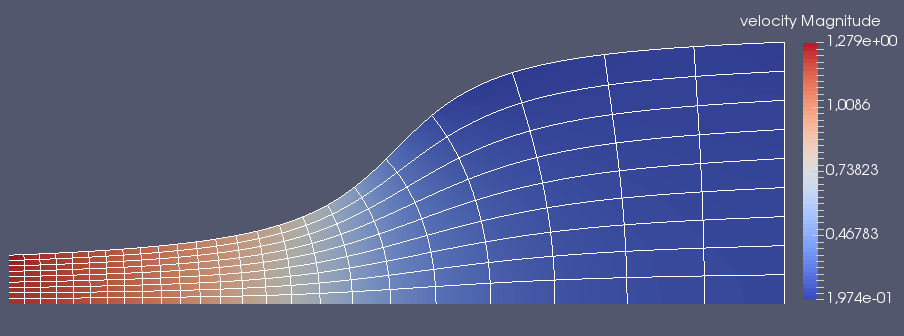
\includegraphics[width=15cm]{bilder/kapitel1/channel1_1}
  \caption{Kanal 1: �quipotential- und Stromlinien}
  \label{fig:channel1_1}
\end{figure}
\FloatBarrier
Es ist ersichtlich, dass sich alle �quipotential- und Stromlinien senkrecht schneiden, so wie es auch aus der Theorie vorgeschrieben wird. Desweiteren stehen die �quipotentiallinien senkrecht auf der Kontur.
\begin{figure}[!htb] 
  \centering
     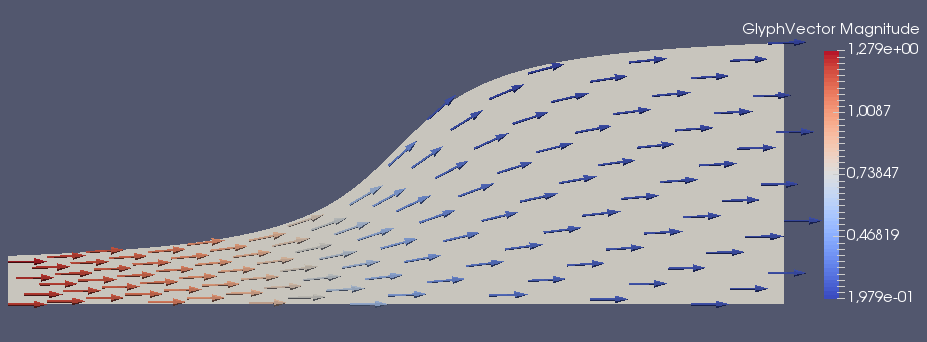
\includegraphics[width=15cm]{bilder/kapitel1/channel1_2}
  \caption{Kanal 1: Geschwindigkeitsfeld}
  \label{fig:channel1_2}
\end{figure}
\begin{figure}[!htb] 
  \centering
     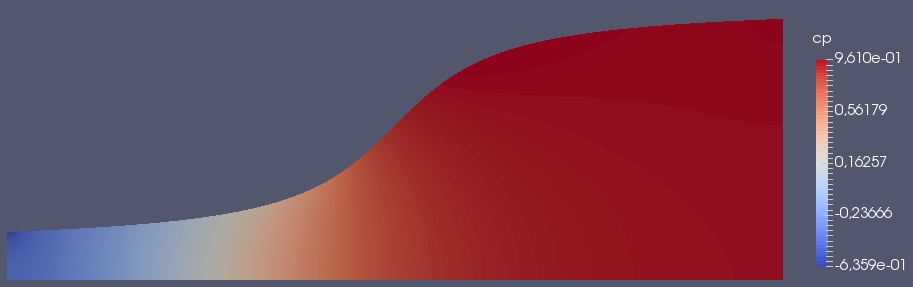
\includegraphics[width=15cm]{bilder/kapitel1/channel1_3}
  \caption{Kanal 1: Druckfeld}
  \label{fig:channel1_3}
\end{figure}
\FloatBarrier
Am Auslauf des Kanals ist der Druckbeiwert bei circa Eins, da $u_{lokal}>u_{\infty}$. Am Einlauf gilt hingegen $u_{lokal}\approx u_{\infty}$, so dass der Druckbeiwert dort ungef�hrt gleich Null ist.
\FloatBarrier

\item
\FloatBarrier
\begin{figure}[!htb] 
  \centering
     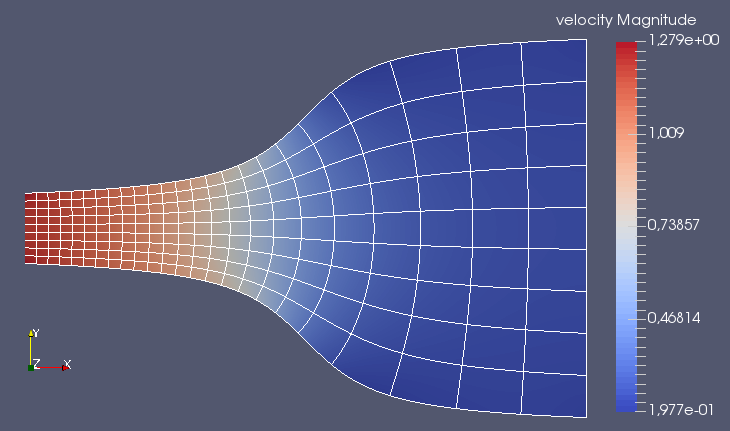
\includegraphics[width=15cm]{bilder/kapitel1/channel2_1}
  \caption{Kanal 2: �quipotential- und Stromlinien}
  \label{fig:channel2_1}
\end{figure}
\FloatBarrier
Es folgen die gleichen Ergebnisse wie bei Kanal 1.
\FloatBarrier
\begin{figure}[!htb] 
  \centering
     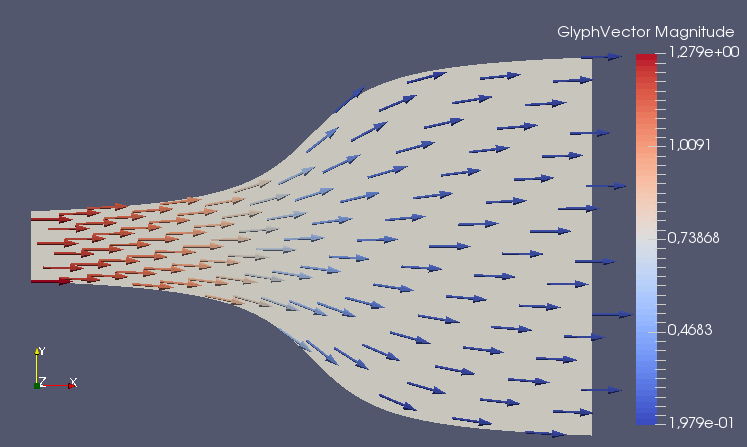
\includegraphics[width=15cm]{bilder/kapitel1/channel2_2}
  \caption{Kanal 2: Geschwindigkeitsfeld}
  \label{fig:channel2_2}
\end{figure}

\item
\FloatBarrier
\begin{figure}[!htb] 
  \centering
     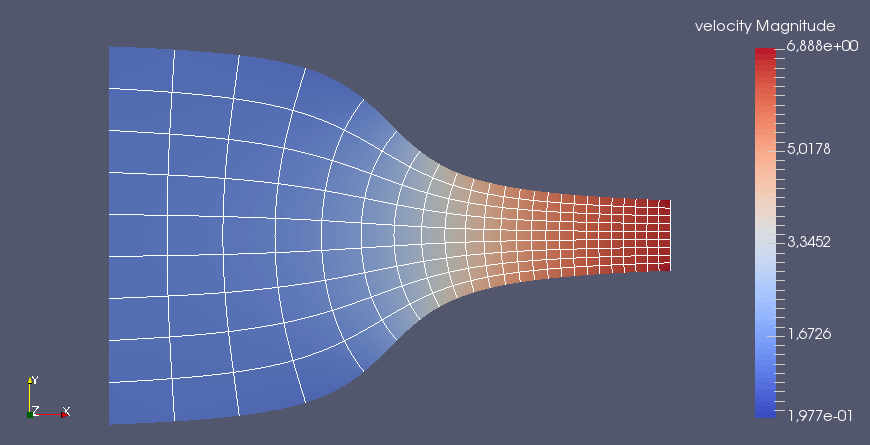
\includegraphics[width=15cm]{bilder/kapitel1/channel3_1}
  \caption{Kanal 3: �quipotential- und Stromlinien}
  \label{fig:channel3_1}
\end{figure}
\FloatBarrier
Es folgen die gleichen Ergebnisse wie bei Kanal 1.
\FloatBarrier
\begin{figure}[!htb] 
  \centering
     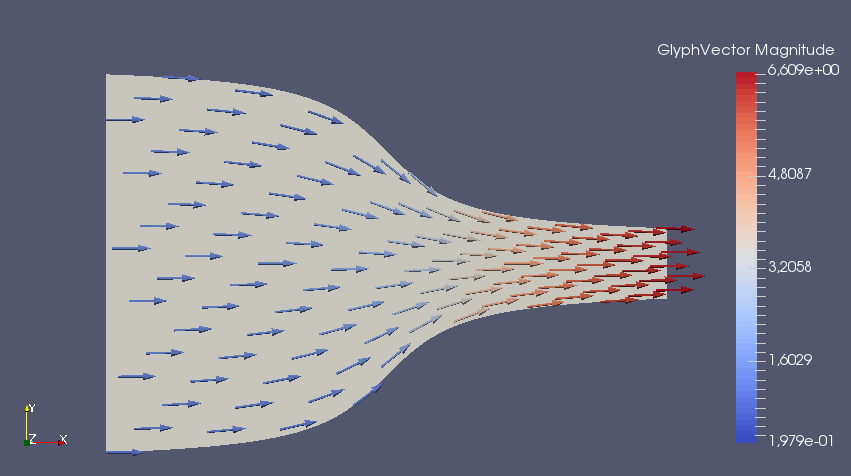
\includegraphics[width=15cm]{bilder/kapitel1/channel3_2}
  \caption{Kanal 3: Geschwindigkeitsfeld}
  \label{fig:channel3_2}
\end{figure}

\item
\FloatBarrier
\begin{figure}[!htb] 
  \centering
     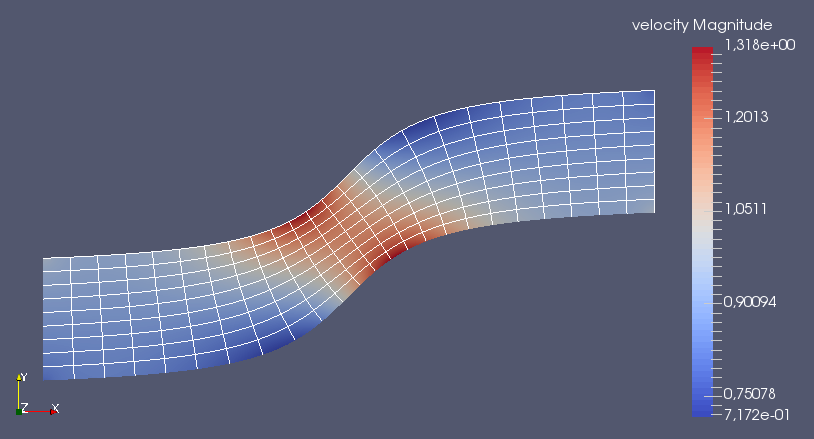
\includegraphics[width=15cm]{bilder/kapitel1/channel4_1}
  \caption{Kanal 4: �quipotential- und Stromlinien}
  \label{fig:channel4_1}
\end{figure}
\FloatBarrier
Es folgen die gleichen Ergebnisse wie bei Kanal 1.
\FloatBarrier
\begin{figure}[!htb] 
  \centering
     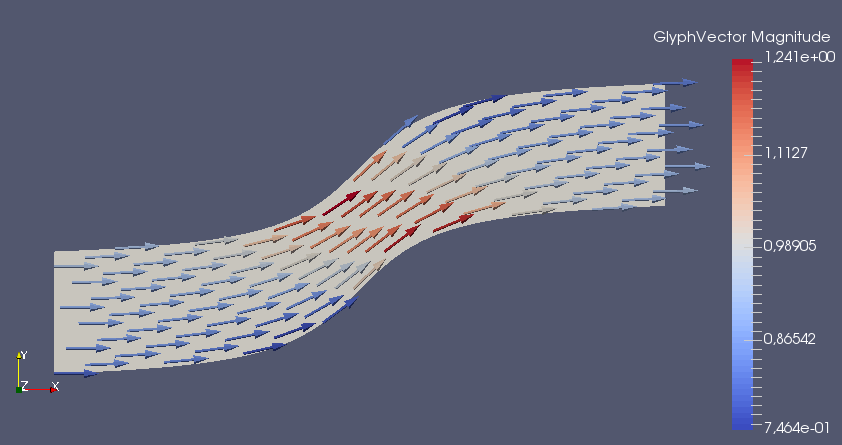
\includegraphics[width=15cm]{bilder/kapitel1/channel4_2}
  \caption{Kanal 4: Geschwindigkeitsfeld}
  \label{fig:channel4_2}
\end{figure}

\end{enumerate}
\FloatBarrier
\underline{\textbf{Bemerkung:}} Die Schnittpunkte aus �quipotentiallinien und Stromlinien bilden ein Gitter auf dem Integrationsgebiet. Somit kann man sich durch Berechnung und Abspeichern dieser Schnittpunkte ein Gitter f�r weitere Diskretisierungen erstellen. Die Knotenpunkte f�r Kanal 2) k�nnten beispielsweise wie folgt aussehen (die Linien mit $\Phi=const$ bzw. $\Psi=const$ sind logarithmisch verteilt, w�re dies nicht der Fall, w�ren die erzeugten Gitterpunkte zum Rand des Kanals hin enger als in der Mitte):
\FloatBarrier
\begin{figure}[!htb] 
  \centering
     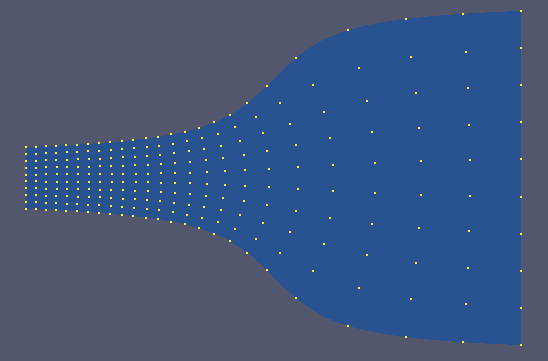
\includegraphics[width=15cm]{bilder/kapitel1/channel2_3}
  \caption{Kanal 2: erzeugtes/berechnetes Gitter}
  \label{fig:channel2_grid}
\end{figure}


\section{Finite Volumen: verschiedene Anwendungsf�lle}

\subsection{Berechnung des Transports eines Skalars}
\subsubsection{Flussstr�mung mit Ein- und Abflussrohr am Rand} \label{sec:fluss}
Betrachtet wird ein Fluss bzw. ein Kanal, welcher station�r mit der selben Geschwindigkeit $u$ in $x$-Richtung flie�t. Am Rand dieses Kanals befindet sich ein Einflussrohr, beispielsweise ein Abfluss einer Fabrik oder ein Zufluss eines anderen Kanals, welches einen Stoff gleicher Dichte $\rho$ in das str�mende Fluid des Kanals gibt. Die Ausstr�mrichtung dieses Rohres steht senkrecht zur Kanalstr�mung. \\
Im Folgenden werden zwei F�lle verglichen:
\begin{itemize}
\item \textbf{Links}: Es wird lediglich ein Stoff in die Kanalstr�mung eingef�hrt.
\item \textbf{Rechts}: Kurz hinter dem Einfluss des neuen Stoffes wird das Fluid des Kanals abgesaugt, ebenfalls am unteren Rand.
\end{itemize}
Die zwei Str�mungen werden an f�nf diskreten Punkten visualisiert. Gerechnet wurde auf einem $100\times50$-Gitter.

\begin{figure}[!htb]
\begin{minipage}[t]{7.8cm}
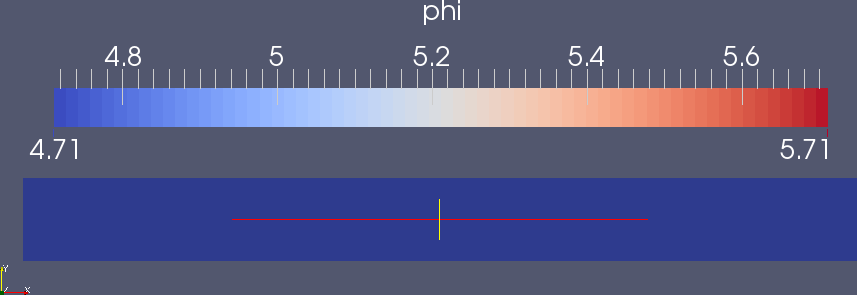
\includegraphics[width=7.7cm]{bilder/anwendungsfaelle/river1_0sek}
\subcaption*{t=$0$ sek}
\end{minipage}
\begin{minipage}[t]{7.8cm}
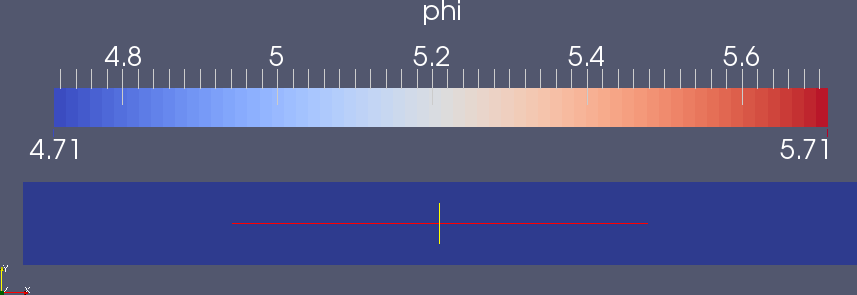
\includegraphics[width=7.7cm]{bilder/anwendungsfaelle/river3_0sek}
\subcaption*{t=$0$ sek}
\end{minipage} \\[0.3cm]
\begin{minipage}[t]{7.8cm}
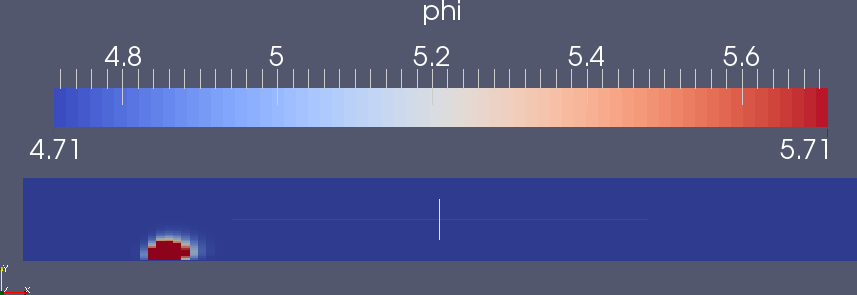
\includegraphics[width=7.7cm]{bilder/anwendungsfaelle/river1_4sek}
\subcaption*{t=$4$ sek}
\end{minipage}
\begin{minipage}[t]{7.8cm}
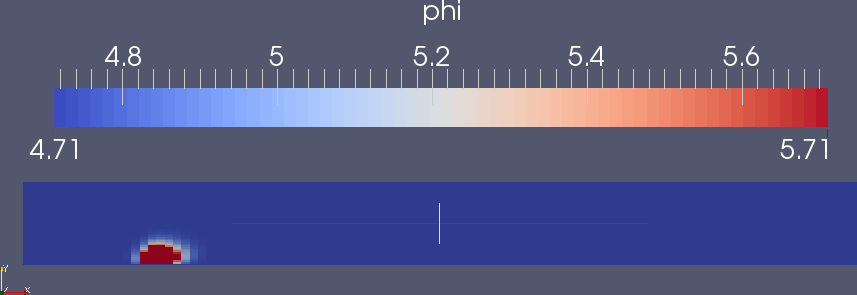
\includegraphics[width=7.7cm]{bilder/anwendungsfaelle/river3_4sek}
\subcaption*{t=$4$ sek}
\end{minipage} \\[0.3cm]
\begin{minipage}[t]{7.8cm}
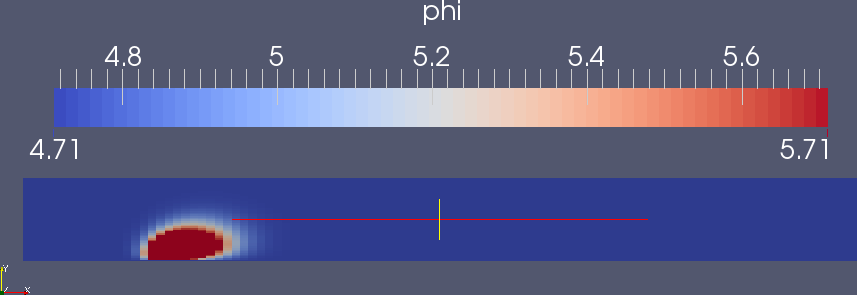
\includegraphics[width=7.7cm]{bilder/anwendungsfaelle/river1_20sek}
\subcaption*{t=$20$ sek}
\end{minipage}
\begin{minipage}[t]{7.8cm}
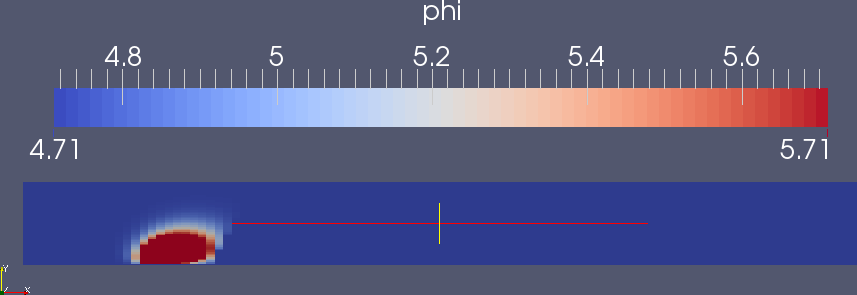
\includegraphics[width=7.7cm]{bilder/anwendungsfaelle/river3_20sek}
\subcaption*{t=$20$ sek}
\end{minipage} \\[0.3cm]
\begin{minipage}[t]{7.8cm}
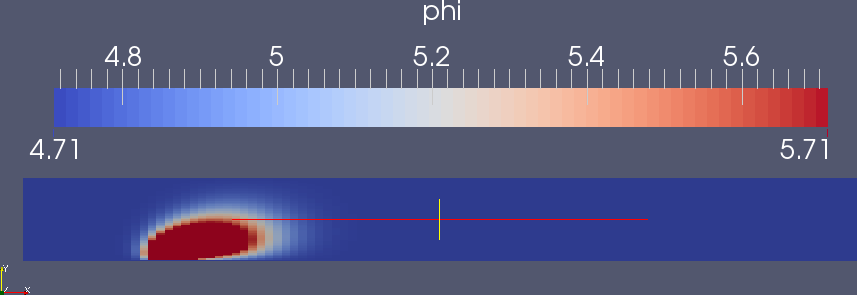
\includegraphics[width=7.7cm]{bilder/anwendungsfaelle/river1_40sek}
\subcaption*{t=$40$ sek}
\end{minipage}
\begin{minipage}[t]{7.8cm}
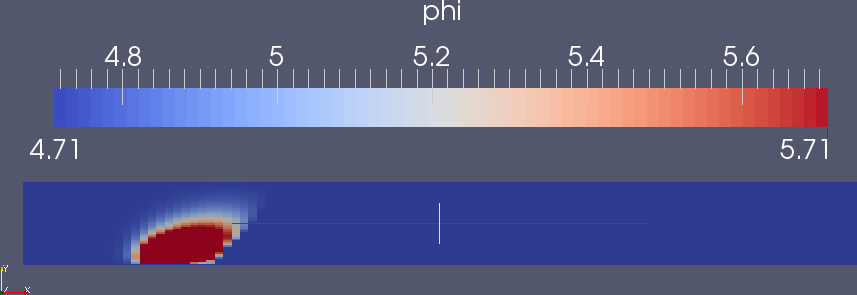
\includegraphics[width=7.7cm]{bilder/anwendungsfaelle/river3_40sek}
\subcaption*{t=$40$ sek}
\end{minipage} \\[0.3cm]
\begin{minipage}[t]{7.8cm}
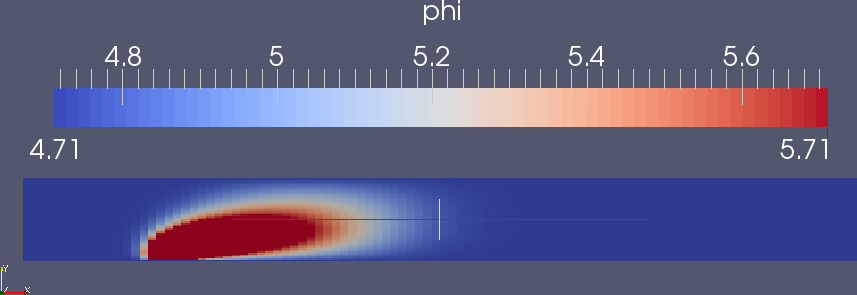
\includegraphics[width=7.7cm]{bilder/anwendungsfaelle/river1_100sek}
\subcaption*{t=$100$ sek}
\end{minipage}
\begin{minipage}[t]{7.8cm}
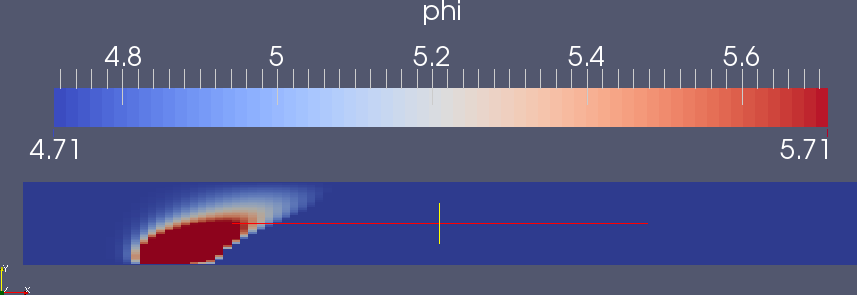
\includegraphics[width=7.7cm]{bilder/anwendungsfaelle/river3_100sek}
\subcaption*{t=$100$ sek}
\end{minipage}
\captionof{figure}{Vergleich Flussstr�mungen: links mit Quelle, rechts mit Quelle und Senke}
\end{figure}
\FloatBarrier

Man erkennt, dass nach $10$ Sekunden der eingef�hrte Stoff von der Kanalstr�mung noch nicht weit genug transportiert wurde, sodass die Zust�nde zu diesem Punkt rechts und links identisch sind. Erst ab circa $20$ Sekunden wird ein Unterschied deutlich. Trotz Quelle bleibt jedoch ein Teil des eingef�hrten Fluids im Kanal verbleiben, da das Einstr�mrohr diesen Stoff so weit in die Mitte des Kanals einstr�mt, dass es nicht komplett von der Senke bzw. dem Abflussrohr wieder abgesogen werden kann.

\subsubsection{Flussstr�mung mit Ein- und Abflussrohr in der Mitte}
Es wird ein �hnlicher Anwendungsfall wie in \ref{sec:fluss} diskutiert. Allerdings befindet sich das Ein- (Quelle) bzw. Abflussrohr (Senke) in der Mitte des Kanals bzw. des Flusses. Es werden drei Ergebnisse gegen�bergestellt:
\begin{itemize}
\item \textbf{Links}:Die Quelle stromauf der Senke f�gt $10\times$ soviel des neuen Fluids hinzu als die Senke absaugt.
\item \textbf{Mitte}:Die St�rke bzw. der Betrag der Ergiebigkeit der Quelle und Senke sind gleich gro�.
\item \textbf{Rechts}:Die Senke stromab der Quelle saugt $10\times$ soviel des neuen Fluids ab als die Quelle hinzuf�gt.
\end{itemize}
Die Simulationseinstellungen bleiben ansonsten die gleichen wie in \ref{sec:fluss}.
\begin{figure}[!htb]
\begin{minipage}[t]{5.6cm}
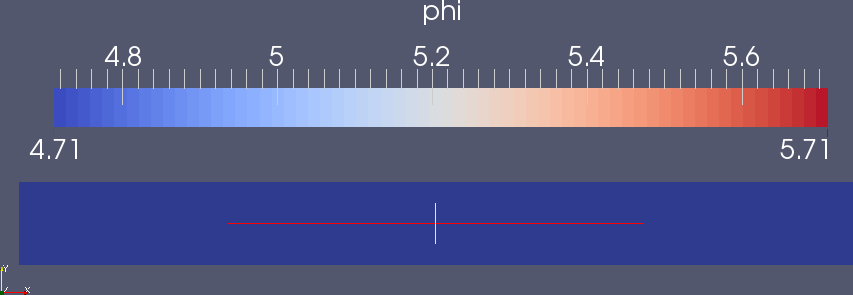
\includegraphics[width=5.5cm]{bilder/anwendungsfaelle/river2_0sek}
\subcaption*{t=$0$ sek}
\end{minipage}
\begin{minipage}[t]{5.6cm}
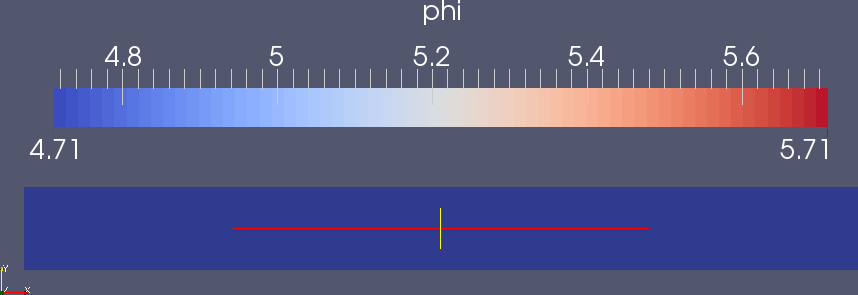
\includegraphics[width=5.5cm]{bilder/anwendungsfaelle/river21_0sek}
\subcaption*{t=$0$ sek}
\end{minipage} 
\begin{minipage}[t]{5.6cm}
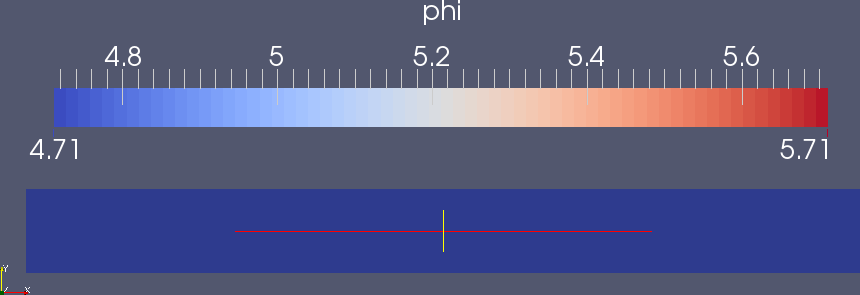
\includegraphics[width=5.5cm]{bilder/anwendungsfaelle/river22_0sek}
\subcaption*{t=$0$ sek}
\end{minipage} \\[0.3cm]
\begin{minipage}[t]{5.6cm}
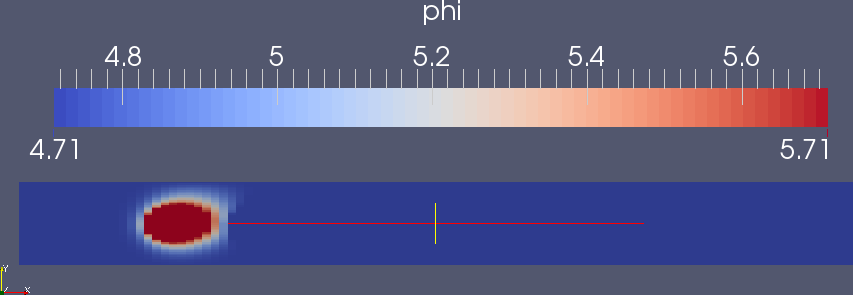
\includegraphics[width=5.5cm]{bilder/anwendungsfaelle/river2_2halfsek}
\subcaption*{t=$2.5$ sek}
\end{minipage}
\begin{minipage}[t]{5.6cm}
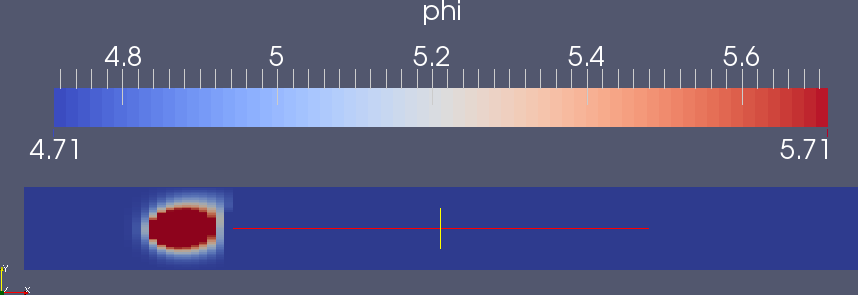
\includegraphics[width=5.5cm]{bilder/anwendungsfaelle/river21_2halfsek}
\subcaption*{t=$2.5$ sek}
\end{minipage} 
\begin{minipage}[t]{5.6cm}
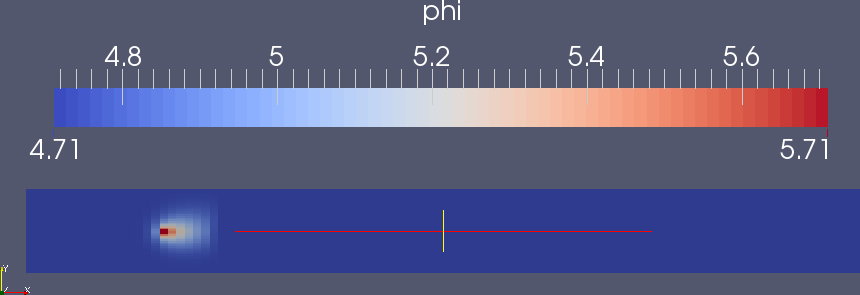
\includegraphics[width=5.5cm]{bilder/anwendungsfaelle/river22_2halfsek}
\subcaption*{t=$2.5$ sek}
\end{minipage} \\[0.3cm]
\begin{minipage}[t]{5.6cm}
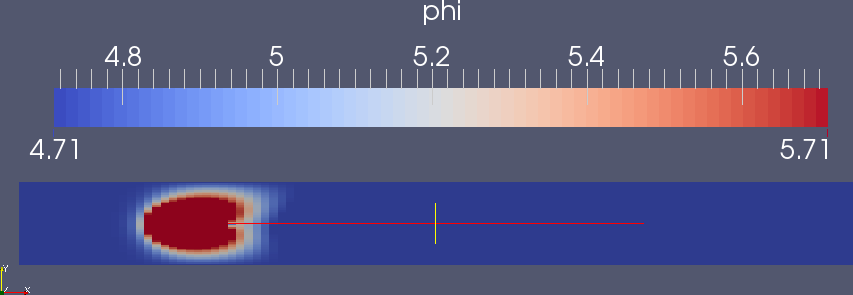
\includegraphics[width=5.5cm]{bilder/anwendungsfaelle/river2_5sek}
\subcaption*{t=$5$ sek}
\end{minipage}
\begin{minipage}[t]{5.6cm}
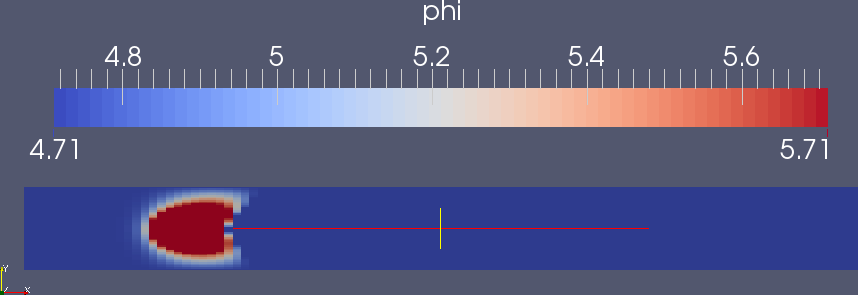
\includegraphics[width=5.5cm]{bilder/anwendungsfaelle/river21_5sek}
\subcaption*{t=$5$ sek}
\end{minipage} 
\begin{minipage}[t]{5.6cm}
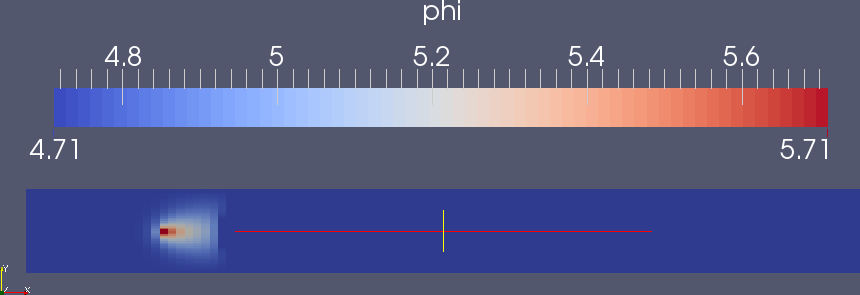
\includegraphics[width=5.5cm]{bilder/anwendungsfaelle/river22_5sek}
\subcaption*{t=$5$ sek}
\end{minipage} \\[0.3cm]
\begin{minipage}[t]{5.6cm}
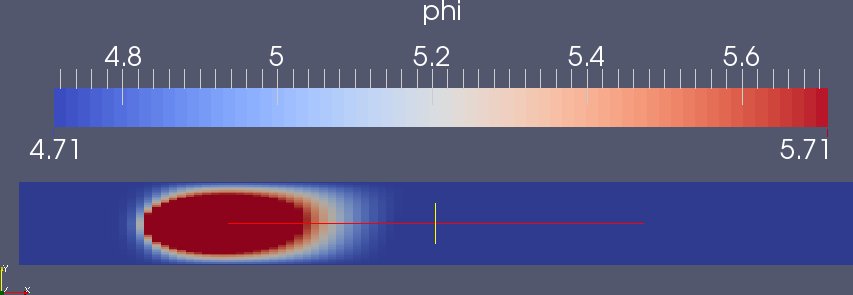
\includegraphics[width=5.5cm]{bilder/anwendungsfaelle/river2_10sek}
\subcaption*{t=$10$ sek}
\end{minipage}
\begin{minipage}[t]{5.6cm}
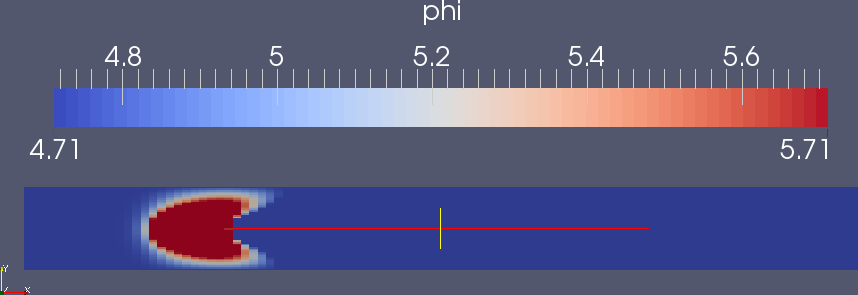
\includegraphics[width=5.5cm]{bilder/anwendungsfaelle/river21_10sek}
\subcaption*{t=$10$ sek}
\end{minipage} 
\begin{minipage}[t]{5.6cm}
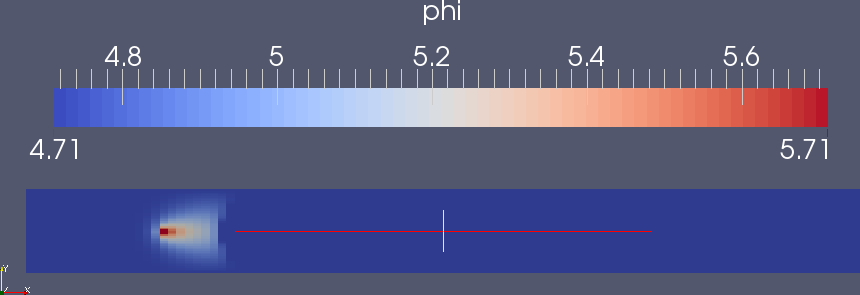
\includegraphics[width=5.5cm]{bilder/anwendungsfaelle/river22_10sek}
\subcaption*{t=$10$ sek}
\end{minipage} \\[0.3cm]
\begin{minipage}[t]{5.6cm}
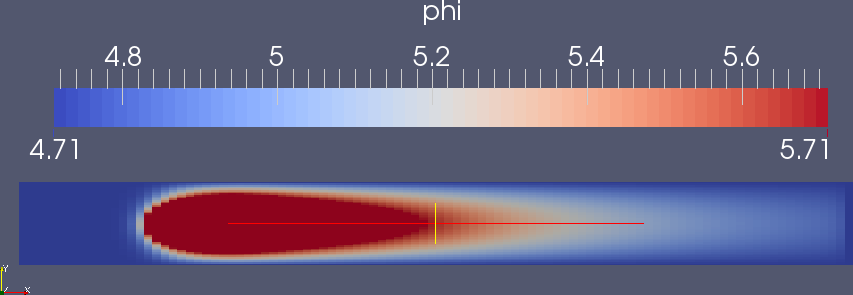
\includegraphics[width=5.5cm]{bilder/anwendungsfaelle/river2_50sek}
\subcaption*{t=$50$ sek}
\end{minipage}
\begin{minipage}[t]{5.6cm}
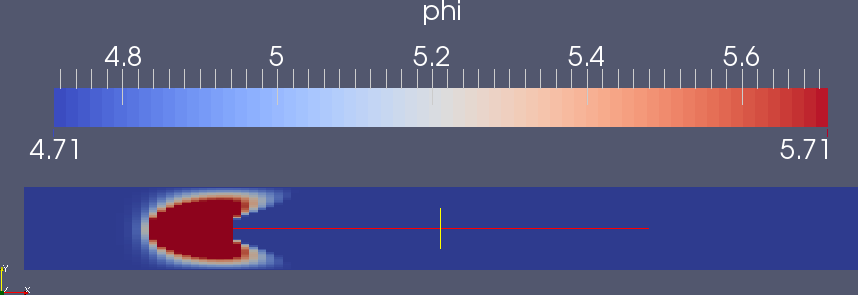
\includegraphics[width=5.5cm]{bilder/anwendungsfaelle/river21_50sek}
\subcaption*{t=$50$ sek}
\end{minipage} 
\begin{minipage}[t]{5.6cm}
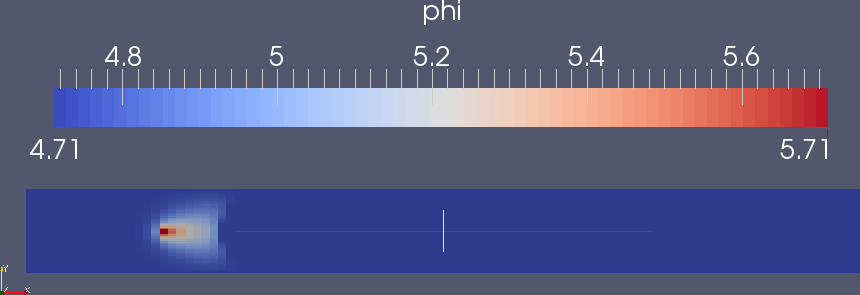
\includegraphics[width=5.5cm]{bilder/anwendungsfaelle/river22_50sek}
\subcaption*{t=$50$ sek}
\end{minipage} \\[0.3cm]
\captionof{figure}{Vergleich Flussstr�mungen: links mit Quelle, rechts mit Quelle und Senke}
\end{figure}
\FloatBarrier

Links wird, aufgrund der st�rkeren Quelle, das neue Fluid entlang des Kanals transportiert, da die Senke \texttt{zu schwach} ist, um es komplett wieder abzusaugen. Hingegen wird beim rechten Fall sogar fast alles aus der Quelle wieder abgesaugt. Hier wird allerdings auch viel Fluid des Flusses abgesaugt. Da die Skala nicht neu skaliert worden ist, wird das hier nicht komplett ersichtlich. Dies ist bewusst gemacht worden, da so zum Einen die drei F�lle besser verglichen werden k�nnen und zum Anderen das Reskalieren den Effekt nicht so deutlich erscheinen l�sst. Gleiches gilt auch f�r die Grafiken aus \ref{sec:fluss}.

\subsection{Berechnung des Geschwindigkeitsfeldes bei gegebenem Druck}
\subsection{Couette-Str�mung}

\subsection{Poiseuille-Str�mung}
\subsection{Berechnung des Druck- und Geschwindigkeitsfeldes mit Hilfe vom \texttt{SIMPLE}-Algorithmus}

% Setze Numerierung wieder auf r�misch zur�ck und setzte von oben fort
% Wert ist demnach der von 'roemisch'
%\newpage
%\pagenumbering{Roman}
%\setcounter{page}{\value{roemisch}}

% Literaturverzeichnis
%\bibliography{literatur/bib}

% Appendix, falls vorhanden
%\appendix
%% Anh�nge, beliebig, kein Zwang
\chapter{Anhang Eins}

\chapter{Anhang Zwei}
% usw ...


% Eidesstattliche Erkl�rung
%% Die eidesstattliche Erkl�rung mit Unterschrift
\chapter*{Erkl�rung der Urheberschaft}

Ich erkl�re hiermit an Eides statt, dass ich die vorliegende Arbeit
ohne Hilfe Dritter und ohne Benutzung anderer als der angegebenen
Hilfsmittel angefertigt habe; die aus fremden Quellen direkt oder
indirekt �bernommenen Gedanken sind als solche kenntlich gemacht. Die
Arbeit wurde bisher in gleicher oder �hnlicher Form in keiner anderen
Pr�fungsbeh�rde vorgelegt und auch noch nicht ver�ffentlicht.


\vspace{4cm}

\hspace{2cm} Ort, Datum \hfill Unterschrift \hspace{2cm}


\end{document}
